%%%%% Please set the path to 'beamer' directory in your environment %%%%%
\newcommand{\beamerDir}[0]{/mnt/c/Users/atsushi/Documents/workspace/env/Beamer/beamer/beamer/}


%%%%% Load setting %%%%%
\documentclass[aspectratio=169, dvipdfmx, 12pt, compress]{beamer}% dvipdfmxしたい

%%%%% Packages %%%%%
\usepackage{bxdpx-beamer}% dvipdfmxなので必要
\usepackage{pxjahyper}% 日本語で'しおり'したい
\usepackage{tikz}
\usepackage{tcolorbox}
\usetikzlibrary{shapes}
\usepackage{xcolor}
\usepackage[absolute,overlay]{textpos}
\usepackage{adjustbox}
\usepackage{caption}
\usepackage{ifthen}


%%%%% Settings %%%%%
\usetheme[sectionpage=progressbar, subsectionpage=progressbar]{metropolis}
% block style
\metroset{block=fill}
% space between line
\renewcommand{\baselinestretch}{1.3}
% space between item
\newlength{\wideitemsep}
\setlength{\wideitemsep}{0.9\itemsep}
% \addtolength{\wideitemsep}{1.0pt} <- more space
\let\olditem\item
\renewcommand{\item}{\setlength{\itemsep}{\wideitemsep}\olditem}
% frame title
\definecolor{coolblack}{rgb}{0.0, 0.18, 0.39}
\setbeamercolor{frametitle}{bg=coolblack!90,fg=white}
\setbeamerfont{frametitle}{size=\large}
\addtobeamertemplate{frametitle}{}{\vspace{-1em}}
\makeatletter
\setlength{\metropolis@frametitle@padding}{1.4ex}% <- default 2.2 ex
% foot line
\addtobeamertemplate{footline}{}{\vspace{-1em}}
% normal text color
\setbeamercolor{normal text}{fg=black!80}
% progress bar
\definecolor{lightgray}{rgb}{0.83, 0.83, 0.83}
\setbeamercolor{progress bar}{bg=lightgray, fg=coolblack}
\setbeamersize{text margin left=15pt, text margin right=15pt}
% equation font
\usefonttheme{professionalfonts}
% Change standard block width
\addtobeamertemplate{block begin}{%
    \centering
    \begin{columns}\begin{column}{0.9\textwidth}
            \centering
            }{}
            \addtobeamertemplate{block end}{}{\end{column}\end{columns}}
% Change alert block width
\addtobeamertemplate{block alerted begin}{%
    \centering
    \begin{columns}\begin{column}{0.9\textwidth}
            \centering
            }{}
            \addtobeamertemplate{block alerted end}{}{\end{column}\end{columns}}
% Change example block width
\addtobeamertemplate{block example begin}{%
    \centering
    \begin{columns}\begin{column}{0.9\textwidth}
            \centering
            }{}
            \addtobeamertemplate{block example end}{}{\end{column}\end{columns}}
% Itemize color
\setbeamertemplate{itemize item}{\color{black}\scriptsize$\blacksquare$}
\setbeamertemplate{itemize subitem}{\color{black}\scriptsize$-$}
% Simplification  color
\definecolor{cobalt}{rgb}{0.0, 0.28, 0.67}
\setbeamercolor{block title example}{fg=black!80,bg=cobalt!35}
\setbeamercolor{block body example}{fg=black,bg=cobalt!15}
% Definition
\BeforeBeginEnvironment{definition}{
    \setbeamercolor{block title}{use=alerted text, bg=alerted text.fg!70,fg=white}
    \setbeamercolor{block body}{use=alerted text, bg=alerted text.fg!20}
}
\AfterEndEnvironment{definition}{% return to default
    \setbeamercolor{block title}{use=structure,fg=structure.fg,bg=structure.fg!20!bg}
    \setbeamercolor{block body}{parent=normal text,use=block title,bg=block title.bg!50!bg, fg=black}
}
% Theorem
\definecolor{seagreen}{rgb}{0.18, 0.55, 0.34}
\setbeamertemplate{theorems}[numbered]
\BeforeBeginEnvironment{theorem}{
    \setbeamercolor{block title}{fg=black!80,bg=seagreen!40}
    \setbeamercolor{block body}{fg=black,bg=seagreen!15}
}
\AfterEndEnvironment{theorem}{% return to default
    \setbeamercolor{block title}{use=structure,fg=structure.fg,bg=structure.fg!20!bg}
    \setbeamercolor{block body}{parent=normal text,use=block title,bg=block title.bg!50!bg, fg=black}
}
% Lemma
\undef{\lemma}
\newtheorem{lemma}{\translate{Lemma}}
\BeforeBeginEnvironment{lemma}{
    \setbeamercolor{block title}{fg=black!80,bg=seagreen!20}
    \setbeamercolor{block body}{fg=black,bg=seagreen!10}
}
\AfterEndEnvironment{lemma}{% return to default
    \setbeamercolor{block title}{use=structure,fg=structure.fg!80,bg=structure.fg!20!bg}
    \setbeamercolor{block body}{parent=normal text,use=block title,bg=block title.bg!50!bg, fg=black}
}


%%%%% Original Command %%%%%
\newcommand{\subt}[1]{\vspace{-2mm}{\fontsize{10pt}{0cm}\selectfont \textcolor{lightgray}{#1}}\vspace{-1mm}}
\newcommand{\lastpage}[0]{\begin{frame}\begin{textblock*}{1.0\linewidth}(0pt, 50pt)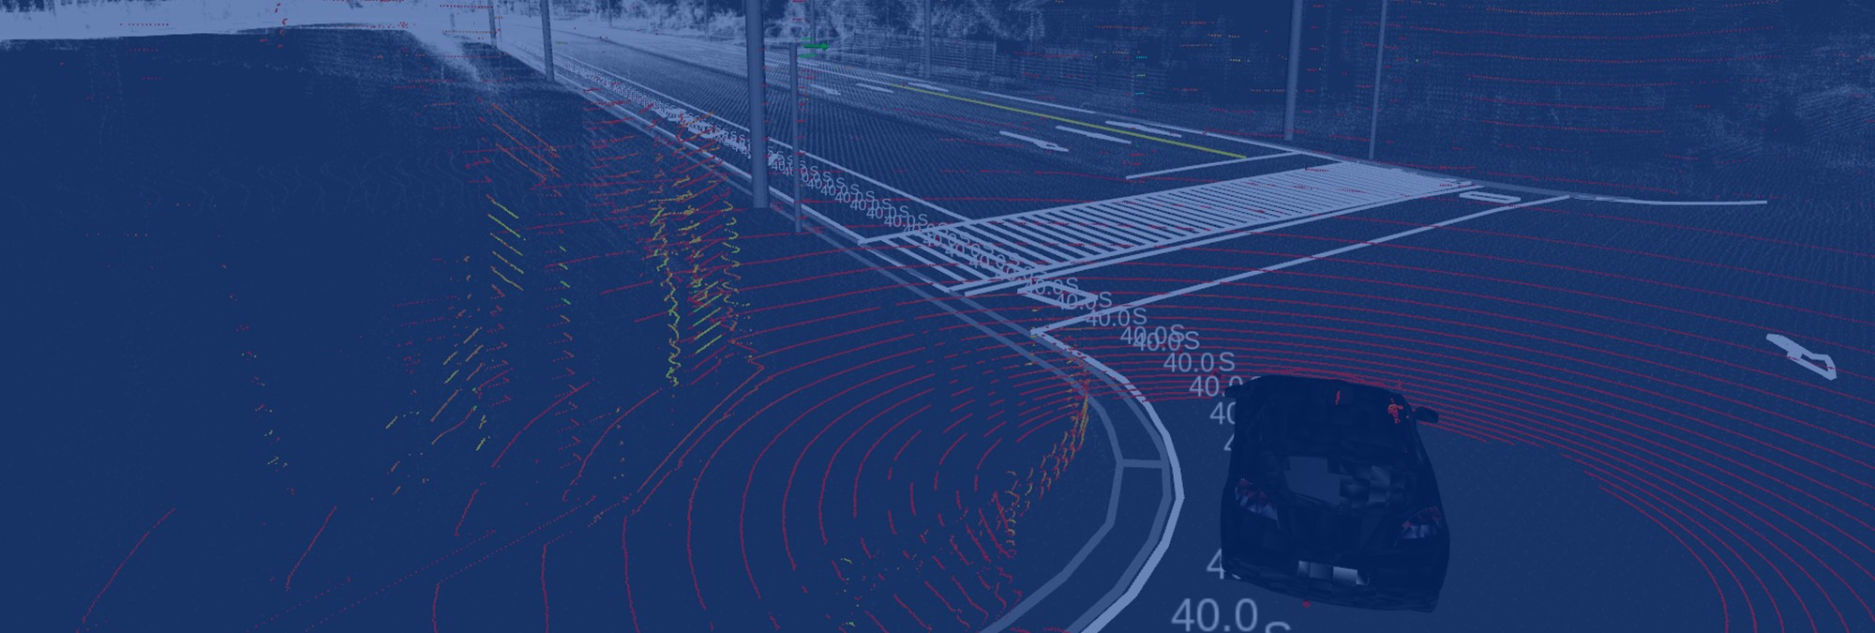
\includegraphics[scale=0.512]{\beamerDir/master_figure/last.pdf}\end{textblock*}\end{frame}}
\newcommand{\todo}[1]{\al{\LARGE\textbf{TODO:} #1}}
\newcommand{\headerheight}[0]{5mm}
\newcommand{\footerheight}[0]{5mm}
\newcommand{\slideheight}[0]{\textheight-\headerheight-\footerheight}
\newcommand{\tabml}[1]{\hspace{-2.1mm}\begin{tabular}{l} #1 \end{tabular}}
\newcommand{\al}[1]{\alert{#1}}
\newcommand{\argempty}[0]{}
\newcommand{\onlyslide}[1]{
    \vspace{\headerheight}
    \begin{minipage}[c][\slideheight][c]{\textwidth}
        #1
    \end{minipage}
}
\newcommand{\onlyimage}[1]{
    \onlyslide{
        \centering
        \begin{columns}
            \begin{column}{\textwidth}
                \centering
                \adjustbox{max width=\textwidth, max height=\slideheight}{
                    \includegraphics{#1}
                }
            \end{column}
        \end{columns}
    }
}
% fit image
\newlength\fitimageht
\newlength\fitotherht
\newsavebox\fitimagebox
\newcommand{\fitimage}[2]{%
    \sbox\fitimagebox{%
        \parbox{\textwidth}{%
            #1\par
        }%
    }%
    \settototalheight{\fitotherht}{%
        \usebox\fitimagebox
    }%
    \setlength\fitimageht{\textheight}%
    \addtolength\fitimageht{-\fitotherht-\headerheight-\footerheight-1\baselineskip}%
    \vspace{\headerheight}
    #1\par
    \centering
    \includegraphics[width=\textwidth,height=\fitimageht,keepaspectratio]{#2}
}
% Simplification
\newcommand{\assume}[1]{
    \begin{exampleblock}{Simplification }
        #1
    \end{exampleblock}
}
% Re-post
\setbeamercolor{RepostBox}{fg=black!50, bg=coolblack!10}
\newcommand{\repost}[1]{
    \vspace{2mm}
    \centering
    \begin{columns}
        \begin{column}{0.86\textwidth}
            \begin{beamercolorbox}[wd=\textwidth, sep=2pt, rounded=true, shadow=true]{RepostBox}
                \begin{tabular}{|p{0.95\textwidth}}
                    {\fontsize{10pt}{10pt}#1}
                \end{tabular}
            \end{beamercolorbox}
        \end{column}
    \end{columns}
}

% equation ballon
\tcbset{
    framebox/.style={
            enhanced,
            boxsep=0pt,       % 箱の上下左右の余白を指定
            colback=white,
            boxrule=1pt,
            colframe=#1
        },
    framebox/.default=red
}
\newcommand{\upbln}[3]{
    \tcboxmath[
        framebox=#2,
        top=0.5ex,bottom=0.5ex,    % 箱の上下の余白を指定
        left=0.5ex,right=0.5ex,    % 箱の左右の余白を指定
        overlay={
                \node[
                    above,
                    rectangle callout,                         % nodeを吹き出しの形に
                    callout absolute pointer={(frame.north)},  % 吹き出しの先端を絶対的に指定
                    fill=#2!20
                ] at ([yshift=2ex]frame.north) {\footnotesize#3};
            }
    ]{#1}
}
\newcommand{\lwbln}[3]{
    \tcboxmath[
        framebox=#2,
        top=0.5ex,bottom=0.5ex,    % 箱の上下の余白を指定
        left=0.5ex,right=0.5ex,    % 箱の左右の余白を指定
        overlay={
                \node[
                    below,
                    rectangle callout,                         % nodeを吹き出しの形に
                    callout absolute pointer={(frame.south)},  % 吹き出しの先端を絶対的に指定
                    fill=#2!20
                ] at ([yshift=-2ex]frame.south) {\footnotesize#3};
            }
    ]{#1}
}
\tcbuselibrary{theorems,skins}



%%%%% Mode %%%%%
% \newcommand{\forme}[1]{#1}
% \newcommand{\forme}[1]{}


%%%%% Front Cover %%%%%
\title{DAG Scheduling and Analysis on Multiprocessor Systems: Exploitation of Parallelism and Dependency}
\subtitle{IEEE Real-Time Systems Symposium (RTSS), 2020}
\author{矢野 篤志}
\date{\today}
\institute[EMBIV]{EMBIV}
\logo{\begin{textblock*}{0.1\linewidth}(2pt, 237pt)
\includegraphics[scale=0.4]{\beamerDir/master_figure/Emb_logo.pdf}\end{textblock*}}


%%%%% Document Start %%%%%
\begin{document}

\maketitle

\summary{1.5}{0}
% !TeX root = main.tex


\begin{frame}{提案の概要}
    \begin{itemize}
        \item 優先度駆動型スケジューリングによってROSのリアルタイム性能と予測可能性を大幅に改善できることを主張する
        \item 主張を裏付けるために, 優先度駆動型チェーン考慮スケジューリングに関する我々の研究をレビューし, Apex.AI が開発したオープンソースリファレンスシステムを用いた評価を行う
        \item ROS 2のリアルタイム性能を向上させるために不可欠な以下2つの課題を説明する
        \begin{itemize}
            \item マルチスレッドエグゼキュータ設計
            \item アクセラレータサポート
        \end{itemize}
    \end{itemize}
\end{frame}


\begin{frame}{Outline}
    \setbeamertemplate{section in toc}[sections numbered]
    \scriptsize\tableofcontents[hideallsubsections]
\end{frame}

% !TeX root = main.tex

\section{PRIOR KNOWLEDGE}
\label{sec: prior knowledge}

\begin{frame}{前提知識}
    \begin{itemize}
        \item \ourl{ROS}{https://tier4.atlassian.net/wiki/spaces/EMBIV/pages/2683603071/ROS+Robot+Operating+System}
        \item \ourl{publish/subscribeモデル}{https://tier4.atlassian.net/wiki/spaces/EMBIV/pages/2675048610/Publish+Subscribe}
        \item \ourl{SCHED\_DEADLINE}{https://tier4.atlassian.net/wiki/spaces/EMBIV/pages/2692645566/SCHED+DEADLINE}
        \item \ourl{最大イベント到着曲線}{https://drive.google.com/file/d/1n85X0vDrDm4IDANDP4aUoC0SNnZLAiRN/view?usp=share_link}
        \item \ourl{Casiniらによる先行研究}{https://drive.google.com/file/d/1sHujFqbmgCoJbC6g6KdC7ihua4Jqddju/view?usp=share_link}
    \end{itemize}
\end{frame}

% !TeX root = main.tex

\section{TASK MODEL AND SCHEDULING PRELIMINARIES}
\label{sec: t}

\begin{frame}{}
    \begin{itemize}
        \item 始めに, 本論文で登場する表記法・用語の表を示す
        \item 基本的な表記法・用語は資料中で説明無しで使用する
        \item 別ファイルで開く・印刷するなどして, 常に参照できる状態にしておくことを推奨する
    \end{itemize}
\end{frame}

% !TeX root = main.tex

\begin{frame}{表記法・用語 1}
    \full{
        \begin{table}[tb]
            \adjustbox{max width=\textwidth, max height=\slideheight}{
                \centering\begin{tabular}{|c|l|} \hline
                    $m$                                                                                             & スレッド数                                                                                        \\\hline
                    $\Gamma=\left\{\mathcal{C}_{1}, \mathcal{C}_{2}, \cdots, \mathcal{C}_{|\Gamma|}\right\}$        & チェインのセット                                                                                  \\\hline
                    $|\Gamma|$                                                                                      & $\Gamma$内のチェインの数                                                                          \\\hline
                    $\mathcal{C}_{i}=\left\{c_{i, 1}, c_{i, 2}, \cdots, c_{i,\left|\mathcal{C}_{i}\right|}\right\}$ & チェイン                                                                                          \\\hline
                    $c_{i,j}$                                                                                       & $\mathcal{C}_{i}$の$j$番目のコールバック                                                          \\\hline
                    $\left|\mathcal{C}_{i}\right|$                                                                  & $\mathcal{C}_{i}$内のコールバックの数                                                             \\\hline
                    先行要素                                                                                        & $J_{i}^{k}$ 内の連続する要素 $c_{i, j}^{k}$ と $c_{i, j+1}^{k}$ の各ペアにおける $c_{i, j}^{k}$   \\\hline
                    後続要素                                                                                        & $J_{i}^{k}$ 内の連続する要素 $c_{i, j}^{k}$ と $c_{i, j+1}^{k}$ の各ペアにおける $c_{i, j+1}^{k}$ \\\hline
                    ソースコールバック                                                                              & $\mathcal{C}_{i}$ の最初のコールバック                                                            \\\hline
                    シンクコールバック                                                                              & $\mathcal{C}_{i}$ の最後のコールバック                                                            \\\hline
                \end{tabular}
            }
        \end{table}
    }
\end{frame}

\begin{frame}{表記法・用語 2}
    \full{
        \begin{table}[tb]
            \adjustbox{max width=\textwidth, max height=\slideheight}{
                \centering\begin{tabular}{|c|l|} \hline
                    $T_i$                 & \tabml{$\mathcal{C}_{i}$の周期                \\\underline{周期}: 2 つの連続するチェーンインスタンスのリリース時刻の間の最小間隔}                       \\\hline
                    $D_i$                 & \tabml{$\mathcal{C}_{i}$の相対デッドライン    \\\underline{相対デッドライン}: 時間 $r$ でリリースされた $\mathcal{C}_{i}$ の各チェーンインスタンスは, \\その絶対デッドライン $r+D_{i}$ までに終了する必要がある}           \\\hline
                    $e_{i,j}$             & $c_{i,j}$の最悪実行時間 (WCET)                \\\hline
                    $E_i$                 & $\mathcal{C}_{i}$内のコールバックのWCETの合計 \\\hline
                    $U_{i}=E_{i} / T_{i}$ & $\mathcal{C}_{i}$の利用率                     \\\hline
                \end{tabular}
            }
        \end{table}
    }
\end{frame}

\begin{frame}{表記法・用語 3}
    \full{
        \begin{table}[tb]
            \adjustbox{max width=\textwidth}{
                \centering\begin{tabular}{|c|l|} \hline
                    $J_{i}^{k}$                & $\mathcal{C}_{i}$ の $k$番目のチェーンインスタンス             \\\hline
                    $c_{i, j}^{k}$             & $J_{i}^{k}$ に含まれる$c_{i, j}$ のコールバックインスタンス    \\\hline
                    $R\left(J_{i}^{k}\right)$  & $J_{i}^{k}$の応答時間                                          \\\hline
                    $\mathcal{R}_i^{wc}$       & $\mathcal{C}_{i}$の最悪応答時間                                \\\hline
                    $\Omega$                   & ready セット                                                   \\\hline
                    $h p\left(c_{i, j}\right)$ & コールバック $c_{i, j}$ よりも優先度の高いコールバックのセット \\\hline
                \end{tabular}
            }
        \end{table}
    }
\end{frame}

\begin{frame}{表記法・用語 4}
    \full{
        \begin{table}[tb]
            \adjustbox{max width=\textwidth, max height=\slideheight}{
                \centering\begin{tabular}{|c|l|} \hline
                    updated  & $\Omega$ に新しい要素が追加されること                                                      \\\hline
                    バッチ   & \tabml{複数のコールバックインスタンスが同じポーリングポイントで $\Omega$ に追加された場合, \\これらのインスタンスは同じバッチである} \\\hline
                    ビジー   & スレッドがコールバックインスタンスが実行している状態                                       \\\hline
                    アイドル & スレッドがコールバックインスタンスを実行していない状態                                     \\\hline
                \end{tabular}
            }
        \end{table}
    }
\end{frame}

\begin{frame}{表記法・用語 5}
    \full{
        \begin{table}[tb]
            \adjustbox{max width=\textwidth, max height=\slideheight}{
                \centering\begin{tabular}{|c|l|} \hline
                    $J$   & 分析対象のチェーン                     \\\hline
                    $r$   & $J$のリリース時刻                      \\\hline
                    $f$   & $J$の終了時刻                          \\\hline
                    $c_i$ & $J$の$i$番目のコールバックインスタンス \\\hline
                    $r_i$ & $c_i$がリリースされる時刻              \\\hline
                    $s_i$ & $c_i$が実行開始する時刻                \\\hline
                    $|J|$ & $J$内のコールバックの数                \\\hline
                \end{tabular}
            }
        \end{table}
    }
\end{frame}


\begin{frame}{表記法・用語 6}
    \full{
        \begin{table}[tb]
            \adjustbox{max width=\textwidth, max height=\slideheight}{
                \centering\begin{tabular}{|c|l|} \hline
                    $\mathcal{S}_{k, i}=\left\langle e_{k, a}^{\prime}, e_{k, b}^{\prime}, \cdots\right\rangle$                                                         & $c_i$に対する$\mathcal{C}_{k}$のサブ干渉シーケンス                                            \\\hline
                    $e_{k, a}^{\prime}$                                                                                                                                 & コールバックインスタンス $c_{k, a}$ が $\left[r_{i}, s_{i}\right)$ の間に実行された時間の長さ \\\hline
                    $\mathcal{S}_{k}=\left\{\mathcal{S}_{k, 1}, \mathcal{S}_{k, 2}, \cdots, \mathcal{S}_{k,|\mathcal{C}|}\right\}$                                      & $J$に対する$\mathcal{C}_{k}$の干渉シーケンス                                                  \\\hline
                    $\mathcal{I}_{k,i}$                                                                                                                                 & $c_i$に対する$\mathcal{C}_{k}$の干渉作業                                                      \\\hline
                    $\mathcal{I}_{k}$                                                                                                                                   & $J$に対する$\mathcal{C}_{k}$の干渉作業                                                        \\\hline
                    $\mathcal{I}_{k,i}^\mathcal{P} $                                                                                                                    & \tabml{$c_i$がブロックされている間に, $c_i$と同じコールバックグループに属す                   \\$\mathcal{C}_k$のコールバックインスタンスが実行した時間の総和} \\\hline
                    $\mathcal{I}_{k,i}^\mathcal{E} $                                                                                                                    & \tabml{$c_i$がブロックされている間に, $c_i$と異なるコールバックグループに属す                 \\$\mathcal{C}_k$のコールバックインスタンスが実行した時間の総和} \\\hline
                    $\mathcal{I}_{k,i}^\mathcal{B}  $                                                                                                                   & \tabml{$[r_i, s_i)$の間に, $c_i$と同じmutually exclusiveコールバックグループに属す            \\$\mathcal{C}_k$のコールバックインスタンスが実行した時間の総和} \\\hline
                    $\mathcal{Q}_{k}=\sum_{i=1}^{|\mathcal{C}|}\left(\mathcal{I}_{k, i}+(m-1) \mathcal{I}_{k, i}^{\mathcal{B}}-\mathcal{I}_{k, i}^{\mathcal{E}}\right)$ & $\mathcal{C}_{k}$の実行が$J$の終了時間に与える影響を特徴付けるために開発した項                \\\hline
                    $\Phi_{k,i}$                                                                                                                                        & $\mathcal{Q}_k$に対する $\mathcal{S}_{k,i}$の寄与                                             \\\hline
                \end{tabular}
            }
        \end{table}
    }
\end{frame}

\begin{frame}{表記法・用語 7}
    \full{
        \begin{table}[tb]
            \adjustbox{max width=\textwidth, max height=\slideheight}{
                \centering\begin{tabular}{|c|l|} \hline
                    $L$                                    & 問題ウィンドウの長さ                                                                                         \\\hline
                    $n_{k}(L)$                             & $J$ の問題ウィンドウ中に実行できる $\mathcal{C}_{k}$ のチェーンインスタンスの最大数                          \\\hline
                    $\overrightarrow{\mathcal{M}}_{k}$     & $J$に対する$\mathcal{C}_{k}$の超干渉シーケンス                                                               \\\hline
                    $ \hat{\Phi} $                         & $\Phi_{k,i}$の上界                                                                                           \\\hline
                    $\mathcal{G}(c_{i,j}) $                & \tabml{$c_{i,j}$が属すmutually exclusiveコールバックグループのインデックス}                                  \\\hline
                    $\theta_i$                             & \tabml{$\mathcal{C}_{i}$ の各コールバックが属すmutually exclusiveコールバックグループの集合                  \\ $\theta_{i}=\cup_{\forall c_{i, j} \in \mathcal{C}_{i}}\left\{\mathcal{G}\left(c_{i, j}\right)\right\}$} \\\hline
                    $\mathcal{I}_{k, i}^{\mathcal{E}^{*}}$ & $\mathcal{S}_{k, i}$ 内の $c_{i}$ とは異なるコールバックグループに属すコールバックインスタンスの合計実行時間 \\\hline
                    $\mathcal{Q}_{k}(\mathcal{Y})$         & 各サブ干渉シーケンス $\mathcal{S}_{k, i}$ に関する $\hat{\Phi}_{k, i}$ の合計                                \\\hline
                \end{tabular}
            }
        \end{table}
    }
\end{frame}

\begin{frame}{表記法・用語 8}
    \full{
        \begin{table}[tb]
            \adjustbox{max width=\textwidth, max height=\slideheight}{
                \centering\begin{tabular}{|c|l|} \hline
                    $\Phi_{k, i}^{p, q}$                            & \tabml{$\overrightarrow{\mathcal{M}}_{k}$ の$ p $番目のコールバックインスタンスの開始時刻から \\$ q $番目のコールバックインスタンスの開始時刻までの \\範囲内にある任意のウィンドウによって発生しうる最大の $\hat{\Phi}_{k, i}$} \\\hline
                    $\left|\overrightarrow{\mathcal{M}}_{k}\right|$ & $\overrightarrow{\mathcal{M}}_{k}$ のコールバックインスタンスの数                             \\\hline
                    $\Theta_{i, p}$ ($i \in[1,|\mathcal{C}|])$      & \tabml{$ p $番目のコールバックインスタンスの開始時刻から                                      \\$\overrightarrow{\mathcal{M}}_{k}$ の最後のコールバックインスタンスの終了時刻までの \\範囲に収まる任意のウィンドウによって発生しうる最大の $\sum_{j=i}^{|\mathcal{C}|} \hat{\Phi}_{k, j}$} \\\hline
                \end{tabular}
            }
        \end{table}
    }
\end{frame}


\begin{frame}{研究対象のモデル}
    単一周期ノンプリエンプティブDAGをホモジニアスマルチプロセッサプラットフォーム上で実行する
\end{frame}

\subsection{Task Model}
\label{ssec: ta}

\begin{frame}{基本の定義1}
    \begin{itemize}
        \item DAGタスク $\tau_{x}$ は, $\left\{T_{x}, D_{x}, \mathcal{G}_{x}=\left(V_{x}, E_{x}\right)\right\}$ で定義され, $T_{x}$ はその最小到着間時間, $D_{x}$ は制約付き相対デッドライン, すなわち $D_{x} \leq T_{x}$, $\mathcal{G}_{x}$ はタスクを形成するアクティビティの集合を定義するグラフとする
        \item グラフは $\mathcal{G}_{x}=\left(V_{x}, E_{x}\right)$ と定義され, $V_{x}$ はノードの集合を示し, $E_{x} \subseteq\left(V_{x} \times V_{x}\right)$ は任意の2つのノードを結ぶエッジの集合を与える
        \item 各ノード $v_{x, j} \in V_{x}$ は, 順次実行されなければならない計算ユニットを表し, その最悪実行時間 (WCET)  $C_{x, j}$ によって特徴付けられる
              \notes{簡単のため, DAGタスクが1つの場合は, DAGタスクの添え字($x$, $\tau_{x}$ など) を省略する}
    \end{itemize}
\end{frame}

\begin{frame}{基本の定義2}
    \begin{itemize}
        \item エッジで結ばれた任意の2つのノード $v_{j}$ と $v_{k}$ に対して, $v_{k}$ は $v_{j}$ が実行を終了している場合にのみ実行を開始できる
        \item $v_{j}$ は $v_{k}$ の先行ノードであり, $v_{k}$ は $v_{j}$ の後続ノードである
        \item ノード $v_{j}$ は, 少なくとも一つの先行ノード $\operatorname{pre}\left(v_{j}\right)$ と少なくとも一つの後続ノード $\operatorname{suc}\left(v_{j}\right)$ を持ち, それぞれ正式には $\operatorname{pre}\left(v_{j}\right)=\left\{v_{k} \in V \mid\left(v_{k}, v_{j}\right) \in E\right\}$ と $\operatorname{suc}\left(v_{j}\right)=\left\{v_{k} \in V \mid\left(v_{j}, v_{k}\right) \in E\right\}$ と定義される
    \end{itemize}
\end{frame}

\begin{frame}{基本の定義3}
    \begin{itemize}
        \item ノード $v_{j}$ の直接または推移的に先行ノードおよび後続ノードであるノードを, それぞれ祖先 $\operatorname{anc}\left(v_{j}\right)$ および子孫 $\operatorname{des}\left(v_{j}\right)$ と呼ぶ
        \item $\operatorname{pre}\left(v_{j}\right)=\varnothing$ または $\operatorname{suc}\left(v_{j}\right)=\varnothing$ を持つノード $v_{j}$ を, それぞれソース $v_{s r c}$, シンク $ v_{s i n k}$ と呼ぶ
        \item 各DAGは1つのソースノードと1つのシンクノードを持つと仮定する
        \item $v_{j}$ と同時実行可能なノードは $\mathcal{C}\left(v_{j}\right)=\left\{v_{k} \mid v_{k} \notin\left(\operatorname{anc}\left(v_{j}\right) \cup \operatorname{des}\left(v_{j}\right)\right), \forall v_{k} \in V\right\}$ で与えられる
    \end{itemize}
\end{frame}

\begin{frame}{パス}
    \begin{block}{パス $\lambda_{a}=\left\{v_{s}, \cdots, v_{e}\right\}$}
        $V$ 内のエッジで接続されたノード列
    \end{block}
    \begin{block}{完全パス}
        ソース $v_{s r c}$ とシンク $v_{s i n k}$を含むパス
    \end{block}
    \begin{block}{パスの長さ $\operatorname{len}\left(\lambda_{a}\right)=\sum_{\forall v_{k} \in \lambda_{a}} C_{k}$}
        パス内のノードのWCETの合計
    \end{block}
    % \item ローカルパスは, タスク内のサブパスであり, ソース $v_{s r c}$ とシンク $v_{s i n k}$ の両方を特徴としていない
\end{frame}

\begin{frame}{クリティカルパス}
    \begin{block}{クリティカルパス $\lambda^{*}$}
        最長の完全パス
    \end{block}
    \begin{block}{クリティカルノード}
        クリティカルパスに含まれるノード
    \end{block}
    \begin{block}{非クリティカルノード $V^{\urcorner}=V \backslash \lambda^{*}$}
        クリティカルノード以外のノード
    \end{block}
    \begin{block}{ワークロード $W=$  $\sum_{\forall v_{k} \in V} C_{k}$}
        DAGタスクの WCET の合計
    \end{block}
    % \item 全ての非クリティカルノードのワークロードを, 非クリティカルワークロードと呼ぶ
\end{frame}


\begin{frame}{DAGタスクの例}
    \begin{columns}
        \begin{column}{0.4\textwidth}
            \begin{itemize}
                \item $\operatorname{pre}\left(v_{7}\right)=\left\{v_{5}, v_{6}\right\}$
                \item $\operatorname{anc}\left(v_{7}\right)=\left\{v_{1}, v_{5}, v_{6}\right\}$
                \item $\operatorname{suc}\left(v_{7}\right)=\operatorname{des}\left(v_{7}\right)=\left\{v_{8}\right\}$
                \item $\mathcal{C}\left(v_{7}\right)=\left\{v_{2}, v_{3}, v_{4}\right\}$
                \item $L=10, W=24$
                \item $\lambda^{*}=\left\{v_{1}, v_{5}, v_{7}, v_{8}\right\}$
                \item $v_{s r c}=v_{1}$, $v_{s i n k}=v_{8}$
            \end{itemize}
        \end{column}
        \begin{column}{0.6\textwidth}
            \fullimage{dag_exam}
        \end{column}
    \end{columns}
\end{frame}


\subsection{Work-Conserving schedule and analysis}
\label{ssec: wc}

\begin{frame}{作業保存型スケジューラ}
    DAGタスクのスケジューリングに関する既存の研究の大部分は, 作業保存型スケジューラを想定する
    \begin{block}{作業保存型スケジューラ}
        保留中のワークロードが存在するときにプロセッサを決してアイドル状態にしないスケジューラ
    \end{block}
\end{frame}

\begin{frame}[label=oldRes]{作業保存型スケジューラの最悪応答時間}
    任意の作業保存型スケジューラでグローバルにスケジューリングされたタスクの最悪応答時間が知られている
    \begin{block}{DAGタスク$\tau_x$の既知の最悪応答時間}
        \begin{equation*}
            R_{x}=L_{x}+\left\lceil\frac{1}{m}\left(W_{x}-L_{x}\right)\right\rceil+\sum_{\tau_{y} \in h p(x)} I_{x, y}
        \end{equation*}
        \begin{itemize}
            \item \desc{$m$}{プロセッサ数}
            \item \desc{$I_{x, y}$}{高優先度DAGタスク $\tau_{y}$ から$\tau_{x}$への干渉}
            \item \desc{$h p(x)$}{$\tau_{x}$以上の優先度を持つDAGタスクセット}
        \end{itemize}
    \end{block}
\end{frame}

\begin{frame}{既知の応答時間の悲観性}
    \begin{itemize}
        \item 既知の分析は, ノード $v_{j}$ が全ての同時実行ノードによって干渉されると仮定しているため悲観的
        \item そこで, 単一DAGタスクの実行時メイクスパンを減らし, 分析的な最悪応答時間を厳しくするための新しい方法を提案する
    \end{itemize}
\end{frame}

% \begin{frame}{}
%     \begin{itemize}
%         \item 図 1(b)は, デュアルコアシステムにおける, 例の DAG の可能な実行シナリオを示したものである
%         \item ノードをランダムにスケジューリングした場合, 合計240の異なる実行シナリオが可能であり, メイクスパンは13から17の範囲である
%         \item 上記の分析により, $R=L+\frac{1}{m}$ ( $W-$  $L)=10+\frac{1}{2}(24-10)=17$ )と安全な境界が得られる
%         \item しかし, 17よりはるかに低いメイクスパンを持つスケジューリングオーダーが存在する
%         \item ジョブ保存スケジュールと古典的な分析に基づいて, 単一の再帰的DAGタスクの実行時メイクスパンを減らし, 分析的な境界を厳しくするための新しい方法を提案する
%     \end{itemize}
% \end{frame}

% !TeX root = main.tex

\section{DAG SCHEDULING: A PARALLELISM AND NODE DEPENDENCY EXPLOITED METHOD}
\label{sec: dag}

\begin{frame}{ヒューリスティック設計方針}
    \begin{itemize}
        \item \hlink{oldRes}{最悪応答時間の式} より, 非クリティカルノードからクリティカルパスへのレイテンシ ($\frac{1}{m}(W-L)$)を最小化することで, DAGのメイクスパンが削減されることが分かる
        \item これをサポートするために, まずノードの依存性と並列性を知るためのCPCモデルを提案する
        \item そして, CPCモデルに基づいてノードの並列度を最大化するスケジューリング手法を示す
    \end{itemize}
\end{frame}

% \begin{frame}{このセクションで使用する表記}
%     \full{
%         \begin{table}[tb]
%             \adjustbox{max width=0.8\textwidth, max height=\slideheight}{
%                 \centering\begin{tabular}{|c|l|} \hline
%                     $\Theta^*$                 & プロバイダ集合                                                                                     \\\hline
%                     $\Theta$                   & コンシューマ集合                                                                                   \\\hline
%                     $\theta_i^*$               & $i$番目のプロバイダ                                                                                \\\hline
%                     $p_j$                      & $\tau_j$の優先度                                                                                   \\\hline
%                     $L_i$                      & $\theta_i^*$の長さ                                                                                 \\\hline
%                     $W_i$                      & $F\left(\theta_i^*\right) \text { and } G\left(\theta_i^*\right)$内のノードの総ワークロード        \\\hline
%                     $\alpha_i$                 & $\theta_i^*$と並列に実行できる$F\left(\theta_i^*\right), G\left(\theta_i^*\right)$内のワークロード \\\hline
%                     $F\left(\theta_i^*\right)$ & $\theta_i^*$のコンシューマ集合                                                                     \\\hline
%                     $G\left(\theta_i^*\right)$ & $\theta_i^*$と並列に実行できる後続プロバイダのコンシューマ集合                                     \\\hline
%                     $f(\cdot)$                 & プロバイダまたはコンシューマの終了時間を返す関数                                                   \\\hline
%                     $l_j(\cdot)$               & $v_j$を含むクリティカルパスの長さを返す関数                                                        \\\hline
%                 \end{tabular}
%             }
%         \end{table}
%     }
% \end{frame}


\subsection{Concurrent Provider and Consumer Model}
\label{ssec: Concurrent provider and consumer model}

\begin{frame}{CPCモデル構築の概要}
    \fitimage{
        CPCモデルは以下のステップで構築される
        \begin{itemize}
            \item クリティカルパスを連続したサブパスの集合に分割する (a)
            \item 各サブパスについて, サブパスと並行して実行でき, 次のサブパスの開始を遅らせる非クリティカルノードを特定する (b ,c)
        \end{itemize}
    }{cpc}
\end{frame}

\begin{frame}{用語の定義}
    \begin{block}{キャパシティ}
        \setlength{\linewidth}{0.98\columnwidth}
        \begin{itemize}
            \item 非クリティカルノードの並列実行に許される時間
            \item クリティカルパスの長さに相当する
        \end{itemize}
    \end{block}
    \begin{block}{キャパシティプロバイダ$\Theta^{*}$}
        クリティカルパスのサブパス
    \end{block}
    \begin{block}{キャパシティコンシューマ$\Theta$}
        全ての非クリティカルノード
    \end{block}
\end{frame}

\begin{frame}{特定のプロバイダに対するコンシューマ}
    \fitimage{
        \begin{block}{$F\left(\theta_{i}^{*}\right)$}
            $\theta_{i}^{*}$ と同時実行可能で, $\theta_{i+1}^{*}$ の開始を遅らせることができるコンシューマ集合
            \[
                F\left(\theta_i^*\right)=\operatorname{anc}\left(\theta_{i+1}^*\right) \cap V^{\neg}
            \]
        \end{block}
    }{f}
\end{frame}

\begin{frame}{後続だが同時実行可能なコンシューマ}
    \fitimage{
        \begin{block}{$G\left(\theta_{i}^{*}\right)$}
            後のプロバイダのコンシューマグループに属すが, $\theta_{i}^{*}$ と並列実行可能なコンシューマ集合
            \[
                G\left(\theta_i^*\right)=\bigcup_{v_j \in F\left(\theta_i^*\right)}\left\{\mathcal{C}\left(v_j\right) \cap V^{\neg}\right\}
            \]
        \end{block}
    }{g}
\end{frame}

\begin{frame}[label=alg1]{CPCモデル構築アルゴリズム全体像}
    \fullimage{cpc_const}
\end{frame}

\begin{frame}{キャパシティプロバイダ特定}
    \fitimage{
        3-9行目で, クリティカルパスと非クリティカルノードの間のノード依存性を分析することにより, キャパシティプロバイダセットを構築する
    }{provider_const}
\end{frame}

\begin{frame}{キャパシティコンシューマ特定}
    \fullimage{consumer}
\end{frame}

\begin{frame}{CPCモデルの利点}
    CPCモデルによって, クリティカルパス上のノードが受ける非クリティカルノードからの直接レイテンシと間接レイテンシの両方について完全な知識を提供する
\end{frame}

% \begin{frame}{}
%     \begin{itemize}
%         \item $F\left(\theta_{i}^{*}\right) \cup G\left(\theta_{i}^{*}\right)$ のノード $v_{j}$ は, $f\left(v_{j}\right) \leq f\left(\theta_{i}^{*}\right)$ または $f\left(v_{j}\right)-C_{j}<f\left(\theta_{i}^{*}\right)$ のいずれかであれば, $\alpha_{i}$ に寄与する
%         \item 前者($\left.f\left(v_{j}\right) \leq f\left(\theta_{i}^{*}\right)\right)$ は $v_{j}$ が $\theta_{i}^{*}$ よりも先に終了し, レイテンシが発生し ないことを示し, 後者($f\left(v_{j}\right)-C_{j}<f\left(\theta_{i}^{*}\right)$)は $v_{j}$ が $\theta_{i}^{*}$ と一部並列実行でき,  $\theta_{i+1}^{*}$ に対するレイテンシが $C_{j}$ よりも少なくなることを示してい る
%     \end{itemize}
% \end{frame}

% \begin{frame}{}
%     \begin{definition}[$\theta_{i}^{*}$ の干渉ワークロード]
%         $\theta_{i}^{*}$ の干渉ワークロードとは, $W_{i}-L_{i}$ において, 時間瞬間 $f\left(\theta_{i}^{*}\right)$ の後に実行されるワークロードのことである
%         プロバイダ $\theta_{i}^{*}$ の場合, その干渉するワークロードは $W_{i}-L_{i}-\alpha_{i}$ である
%     \end{definition}
% \end{frame}

% \begin{frame}[label=lemma1]{Lemma 1}
%     \begin{lemma}[]
%         プロバイダ $\theta_{i}^{*}$ と $\theta_{i+1}^{*}$ に対して, $\theta_{i+1}^{*}$ の開始を遅らせることができる $W_{i}$ のワークロードは, 最大で $W_{i}-L_{i}-\alpha_{i}$ である
%     \end{lemma}
% \end{frame}


\subsection{The “Critical Path First” execution (CPFE)}
\label{ssec: CPEF}

% \begin{frame}{}
%     \begin{itemize}
%         \item CPCモデルでは, クリティカルパスは概念的に容量提供者の集合としてモデル化される
%         \item 各完全パスは, 他のノードが並列実行できるようにパス長の時間間隔を提供するプロバイダと見なすことができる
%         \item しかし, クリティカルパスは最大容量を提供するため, 最大限の並列ワークロード($\alpha=$  $\sum_{\theta_{*}^{*} \in \Theta^{*}} \alpha_{i}$ と表記) を可能にする
%         \item これにより, 完全なクリティカルパス上で干渉するワークロードを最小化するためのプラットフォームが提供される
%     \end{itemize}
% \end{frame}

\begin{frame}[label=theorem1]{クリティカルパス優先の最適性}
    \begin{theorem}[]
        クリティカルパスを最優先にスケジュールするアルゴリズム $\mathcal{S}$ と, \\他の完全パスを優先するアルゴリズム $\mathcal{S}^{\prime}$ において, \\$\mathcal{S}$ の総並列ワークロードは $\mathcal{S}^{\prime}$ 以上である
        \notes{証明略}
    \end{theorem}

    \setbeamercolor{block title}{fg=black!80,bg=black!15}
    \setbeamercolor{block body}{fg=black!80,bg=white}
    \begin{block}{$\theta_{i}^{*}$ の並列ワークロード}
        $\theta_{i}^{*}$ の並列ワークロードは, $W_{i}-L_{i}$ において, 時間瞬間 $f\left(\theta_{i}^{*}\right)$ より前に実行可能なワークロード
    \end{block}
\end{frame}

\begin{frame}{パスの優先度決定方法}
    \hlink{theorem1}{Theorem 1}に基づき, CPFEのルール1が導かれる
    \begin{definition}[ルール1]
        クリティカルノードに最も高い優先度を割り当てる
        \[
            \forall v_{j} \in \Theta^{*}, \forall v_{k} \in \Theta \Rightarrow p_{j}>p_{k}
        \]
    \end{definition}
\end{frame}


\subsection{Exploiting parallelism and node dependency}
\label{ssec: Exploiting parallelism and node dependency}

\begin{frame}{コンシューマ集合の優先度決定方法}
    既存手法\cite{he2019intra}に則り, CPFEはルール2を採用
    \begin{definition}[ルール2]
        より前に位置するプロバイダに対するコンシューマを優先する
        $\forall \theta_{i}^{*}, \theta_{l}^{*} \in \Theta^{*}: i<l \Rightarrow \min _{v_{j} \in F\left(\theta_{i}^{*}\right)} p_{j}>\max _{v_{k} \in F\left(\theta_{l}^{*}\right)} p_{k}$
    \end{definition}
\end{frame}

\begin{frame}{コンシューマ集合内の優先度決定方法}
    既存手法\cite{he2019intra}に則り, CPFEはルール3を採用
    \begin{definition}[ルール3]
        コンシューマが属すパスが長いほど, 高い優先度を割り当てる
        \[
            v_{j}, v_{k} \in F\left(\theta_{i}^{*}\right): l_{j}\left(F\left(\theta_{i}^{*}\right)\right)>l_{k}\left(F\left(\theta_{i}^{*}\right)\right) \Rightarrow p_{j}>p_{k}
        \]
        \vspace{-3mm}
        \begin{itemize}
            \item \desc{$l_{j}\left(F\left(\theta_{i}^{*}\right)\right)$}{$F\left(\theta_{i}^{*}\right)$ のうち $v_{j}$ を含むクリティカルパスの長さ}
        \end{itemize}
    \end{definition}
\end{frame}

% \begin{frame}{}
%     \begin{itemize}
%         \item しかし, 各 $F\left(\theta_{i}^{*}\right)$ にルール3を適用するだけでは十分ではない
%         \item 複雑なDAG構造が与えられた場合, 全ての $F\left(\theta_{i}^{*}\right)$ はより小さなDAG $\mathcal{G}^{\prime}$ を形成することができ, したがって, $F\left(\theta_{i}^{*}\right)$ のクリティカルパスを持つ内側の入れ子CPCモデルが提供者となる
%         \item さらに, この手順を再帰的に適用して, コンシューマグループ内の全てのローカルパスが完全に独立になるまで, 入れ子CPCモデル内の各コンシューマグループに対して内側CPCモデルを構築し続けることができる
%         \item 各内部ネスト CPC モデルでは, ルール 1 とルール 2 を適用して各コンシューマグループの容量を最大化し, レイテンシを最小化する必要があるが, ルール 3 はコンシューマグループの独立したパスにのみ適用して並列性を最大化する (従って, ルール 3 には星マークが付きます)
%         \item これにより, ノード間の依存関係を完全に認識し, 各ネストしたCPCモデルにおいてクリティカルパスを最初に保証できる
%     \end{itemize}
% \end{frame}

\begin{frame}[label=alg2]{CPFE全体像}
    \fullimage{cpef}
\end{frame}

\begin{frame}{CPEF補足1}
    \fullimage{alg2_sup1}
\end{frame}

\begin{frame}{CPEF補足2}
    \fullimage{alg2_sup2}
\end{frame}

\begin{frame}{提案の流れまとめ}
    \begin{enumerate}
        \item \hlink{alg1}{DAGのCPCへの変換}
        \item \hlink{alg2}{各ノードへのルールベース静的優先度割り当て}
        \item 固定優先度スケジューラによるDAGの実行
    \end{enumerate}
\end{frame}

% !TeX root = main.tex

\section{$(\alpha, \beta)$-PAIR RESPONSE TIME ANALYSIS}
\label{sec: RESPONSE TIME ANALYSIS}

\begin{frame}{}
    \begin{itemize}
        \item 本資料では, 分析方法のみを示す
        \item 証明は論文を参照
    \end{itemize}
\end{frame}

\begin{frame}{DAGタスクの応答時間分析}
    DAGタスクの最悪応答時間は以下の式で導出可能
    \[
        \min \left\{R, L+\left\lceil\frac{1}{m}(W-L)\right\rceil\right\}
    \]
    ここで,
    \begin{equation*}
        R=\sum_{\theta_{i}^{*} \in \Theta^{*}}\left\{L_{i}+\left\lceil\frac{1}{m}\left(W_{i}-L_{i}-\alpha_{i}-\beta_{i}\right)\right\rceil+\beta_{i}\right\}
    \end{equation*}
    % 提案する分析は必ずしも従来の境界を支配しているわけではないため, $\min \left\{R, L+\left\lceil\frac{1}{m}(W-L)\right\rceil\right\}$ を最終的な分析的な境界とする
\end{frame}

\begin{frame}{$\alpha, \beta$計算方法}
    \fullimage{a_b}
\end{frame}

% \subsection{The $(\alpha, \beta)$-pair analysis formulation}
% \label{ssec: a}

% \begin{frame}{}
%     \begin{itemize}
%         \item CPC モデルでは, DAG タスクのクリティカルパスは, 連続し たプロバイダ $\Theta^{*}$ の集合に転送される
%         \item プロバイダ $\theta_{i}^{*} \in \Theta^{*}$ は, 前のプロバイダ $\theta_{i-1}^{*}$ とそのコンシューマ $F\left(\theta_{i-1}^{*}\right)$ が実行を終了した場合にのみ開始できる (図2 (b) )
%         \item また, $F\left(\theta_{i-1}^{*}\right)$ は $G\left(\theta_{i-1}^{*}\right)$  (すなわち, $F\left(\theta_{i-1}^{*}\right)$ と同時実行可能な早期リリースされたコンシューマ) からのレイテンシを受けることができ, その結果, $\theta_{i}^{*}$ の開始がレイテンシする (図2 (c) )
%     \end{itemize}
% \end{frame}

% \begin{frame}{}
%     \begin{itemize}
%         \item 定義 1 および 2 に基づき, $\theta_{i}^{*}$ の並列ワークロード $\alpha_{i}$ は, $m-1$ コアの $f\left(\theta_{i}^{*}\right)$ よりも遅く終了しない
%         \item $\theta_{i}^{*}$ が完了した後, 干渉ワークロード (存在する場合) が全ての $m$ コアで実行され, $F\left(\theta_{i}^{*}\right)$ の最新終了ノードが, 次のプロバイダ (存在する場合) に最も早い開始時刻を提供する
%     \end{itemize}
% \end{frame}

% \begin{frame}{}
%     そのため, 以下の上界が必要
%     \begin{enumerate}
%         \item  は, 並列ワークロードの境界 (すなわち, $\alpha_{i}$ )である

%         \item  $F\left(\theta_{i}^{*}\right)$ において, $f\left(\theta_{i}^{*}\right)$ よりも後に実行される (すなわち, 干渉するワークロードにおいて) 最長の実行 シーケンスに対する境界($\beta_{i}$ と表記する)

%     \end{enumerate}
% \end{frame}


\subsection{Supporting explicit execution order}
\label{ssec: Supporting explicit execution order}

\begin{frame}{本セクションの概要}
    \begin{itemize}
        \item これまでの分析は, 明示的な実行順序が事前に分かっていることは想定していない
        \item 非クリティカルノードの明示的な実行順序を使用すると, 各ノードがより高い優先度を持つ同時実行ノードからの干渉しか受けないため, より厳しい境界を得ることができる
        \item そこで, 提案スケジューリングで得られる明示的な実行順序をサポートできるように分析を拡張する
    \end{itemize}
\end{frame}

\begin{frame}{実行順序があるDAGタスクの最悪応答時間計算方法}
    \fullimage{r_order}
\end{frame}

% \begin{frame}{}
%     \begin{itemize}
%         \item ノード優先度を用いると, $m-1$ コアの $v_{j}$ の干渉ノードは, 1) $p_{j}\cite{he2019intra}$ より優先度の高い $\mathcal{I}\left(v_{j}\right)$ のノード, 2) $\mathcal{I}\left(v_{j}\right)$ の優先度が低くノンプリエンプティブスケジュールにより最も WCET の高いノードに効率よく削減できる[10]
%         \item $\mathcal{I}^{e}\left(v_{j}\right)$ は, 非クリティカルなノード $v_{j}$ を明示的な順序で妨害できるノードを示すと, それは式10のように与えられ, この中で $\operatorname{argmax}{ }_{v_{k}}^{m-1}$ は与えられたメトリック $\left(C_{k}\right.$ の値が最も高い最初の $m-1$ ノードを返す)
%         \item この式の正しさは\cite{he2019intra}および[10]で証明されている
%     \end{itemize}
% \end{frame}

% \begin{frame}{}
%     \begin{itemize}
%         \item 簡単のために, $(m-1)$ の低優先度ノードを安全な上界とする
%         \item このブロッキングを正確に計算するために, より細かいILPベースのアプローチが[10]で利用可能である
%         \item さらに, ノードレベルの先取りが許される場合, $\mathcal{I}^{e}\left(v_{j}\right)$ はさらに $\left\{v_{k} \mid p_{k}>p_{j}, v_{k} \in \mathcal{I}\left(v_{j}\right)\right\}$ に縮小される

%               \begin{equation*}
%                   \begin{aligned}
%                       \mathcal{I}^{e}\left(v_{j}\right)=\left\{v_{k} \mid p_{k}>p_{j}, v_{k} \in \mathcal{I}\left(v_{j}\right)\right\} \cup \\
%                       \underset{v_{k}}{\operatorname{argm}} \underset{m}{m a x}\left\{C_{k} \mid p_{k}<p_{j}, v_{k} \in \mathcal{I}\left(v_{j}\right)\right\}
%                   \end{aligned}
%               \end{equation*}
%     \end{itemize}
% \end{frame}

% \begin{frame}{}
%     \begin{itemize}
%         \item このスケジュールでは, $f\left(v_{j}\right), \forall v_{j} \in V$ は式 3 で計算され, $\mathcal{I}^{e}\left(v_{j}\right)$ は $m-1$ コアで実行される非クリティカルノードに適用されま す
%         \item したがって, $\alpha_{i}$ と $\beta_{i}$ は, それぞれ式7と式9により, 更新された $f\left(\theta_{i}^{*}\right)$ と $f\left(v_{j}\right), \forall v_{j} \in F\left(\theta_{i}^{*}\right) \cup G\left(\theta_{i}^{*}\right)$ で境界を設定できる
%         \item 式8で計算される明示的なスケジュール $\lambda_{v_{e}}$ では, 干渉するワークロードで実行される $F\left(\theta_{i}^{*}\right)$ の最長のパスとは限らないことに注意すること\cite{he2019intra}
%         \item その代わり, この場合の $\lambda_{v_{e}}$ は, 事前に計画されたノードの実行順序により, 常に最後に終了するパスを与え ます
%     \end{itemize}
% \end{frame}

% \begin{frame}{}
%     \begin{itemize}
%         \item しかし, DAGタスクの応答時間に関する最終的な境界は, 一般的な場合, すなわち, 式2とは異なっている
%         \item ノード優先では, $\left(W_{i}-\right.$  $L_{i}-\alpha_{i}-\beta_{i}$ )内の全てのワークロードが $\lambda_{v_{e}}$ の実行を妨げることができる必要はない
%         \item $R^{e}$ は, 明示的なスケジューリング順序を持つDAGタスクの応答時間であるとする
%         \item $\mathcal{I}^{e}\left(\lambda_{v_{e}}\right)$ は $\lambda_{v_{e}}$ をレイテンシさせることができるノードを決定し, $I_{\lambda_{v_{e}}, j}$ は干渉するワークロードのノード $v_{j}$ から $\lambda_{v_{e}}$ 上の実際のレイテンシを与える式11で束縛される
%               \[
%                   R^{e}=\sum_{\theta_{i}^{*} \in \Theta^{*}} L_{i}+\beta_{i}+ \begin{cases}0, & \text { if }\left|\Lambda_{\mathcal{I}^{e}\left(\lambda_{v_{e}}\right)}\right|<m \\ {\left[\frac{1}{m} \times \sum_{v_{j} \in \mathcal{I}^{e}\left(\lambda_{v_{e}}\right)}\right.} & \left.I_{\lambda_{v_{e}}, j}\right], \text { otherwise }\end{cases}
%               \]
%     \end{itemize}
% \end{frame}

% \begin{frame}{}
%     \begin{itemize}
%         \item $\theta_{i}^{*}\left(L_{i}\right)$ の長さと, 干渉するワークロードの $\lambda_{v_{e}}\left(\mathrm{I}_{\lambda_{v_{e}}}\right)$ の最悪レイテンシを考えると, $\theta_{i}^{*}$ と $F\left(\theta_{i}^{*}\right)$ の最悪終了時間は $L_{i}+\beta_{i}+$  $\left[\frac{1}{m} \times \sum_{v_{j} \in \mathcal{I}^{e}\left(\lambda_{v_{e}}\right)} I_{\lambda_{v_{e}}, j}\right]$ で上界が決まっている
%         \item また, $\mathrm{I}_{\lambda_{v_{e}}}$ を発生させうるノード内のパス数が $m$ より少ない場合 (すなわち, $\left.\left|\Lambda_{\mathcal{I}^{e}\left(\lambda_{v_{e}}\right)}\right|<m\right), \lambda_{v_{e}}$ が $\theta_{i}^{*}$ の直後に実行され, $L_{i}+\beta_{i}$ までに終了する場合
%         \item このことは, Lemma 3 で証明されている
%         \item $F\left(\theta_{i}^{*}\right)$ の全てのワークロードが $\alpha_{i}$ に寄与するため, $\mathrm{I}_{\lambda_{v_{e}}}=0$ が $\beta_{i}=0$ の場合, $\theta_{i+1}^{*}$  (存在する場合) は $\theta_{i}^{*}$ の直後に開始できることに注意する必要がある
%     \end{itemize}
% \end{frame}

% \begin{frame}{}
%     \begin{itemize}
%         \item $\lambda_{v_{e}}$ に干渉できるノード (すなわち, $\mathcal{I}^{e}\left(\lambda_{v_{e}}\right)$ )は, 式 12 で与えられ, この中で $I_{\lambda_{v_{e}, j}}$ は, ノード $v_{j}$ から $\lambda_{v_{e}}$ への実際のレイテンシを与える
%               \begin{equation*}
%                   \begin{array}{r}
%                       \mathcal{I}^e\left(\lambda_{v_e}\right)=\bigcup_{v_k \in \lambda_{v_e}}\left\{v_j \mid f\left(v_j\right)>f\left(\theta_i^*\right) \wedge p_j>p_k, \forall v_j \in \mathcal{I}\left(v_k\right)\right\} \cup \\
%                       \bigcup_{v_k \in \lambda_{v_e}} \operatorname{argmmax}\left\{\begin{array}{c}
%                                                                                        1. m \\
%                                                                                        v_k
%                                                                                    \end{array}\left\{I_{\lambda_{v_e}, j} \mid f\left(v_j\right)>f\left(\theta_i^*\right) \wedge p_j<p_k, v_j \in \mathcal{I}\left(v_k\right)\right\}\right.
%                   \end{array}
%               \end{equation*}
%     \end{itemize}
% \end{frame}

% \begin{frame}{}
%     最後に, $I_{\lambda_{v_{e}}, j}$ は, $f\left(\theta_{i}^{*}\right)$ の後に実行される $v_{j}$ のワークロード (すなわち, 干渉ワークロード) を $\lambda_{v_{e}}$ の最悪レイテンシとする式13で拘束される

%     \begin{equation*}
%         I_{\lambda_{v_{e}}, j}= \begin{cases}C_{j}, & \text { if } f\left(v_{j}\right)-C_{j} \geq f\left(\theta_{i}^{*}\right) \\ f\left(v_{j}\right)-f\left(\theta_{i}^{*}\right), & \text { otherwise }\end{cases}
%     \end{equation*}
% \end{frame}

% \begin{frame}{}
%     \begin{itemize}
%         \item これで, ノードの実行順序が事前に分かっているスケジューリング手法の分析は終了である
%         \item 一般的な境界と同様に, 任意のノードの WCET を削減しても, 最悪境界より遅い完了には至らないため, この分析は持続可能である (セクション IV-A を参照)
%         \item ランダムな順序の非重要ノードに対する一般的な境界と比較して, この分析では, $\mathcal{I}^{e}\left(v_{j}\right) \subseteq \mathcal{I}\left(v_{j}\right)$ と $\mathrm{I}_{v_{e}} \leq W_{i}-L_{i}-\alpha_{i}-\beta_{i}$ という優先度によりレイテンシを引き起こすことができないノードを取り除くことにより, よりタイトな結果を得ることができる
%     \end{itemize}
% \end{frame}

% \begin{frame}{}
%     \begin{itemize}
%         \item さらに, 提案する分析は, 特定のスケジュールに対して\cite{he2019intra}の分析を厳密には支配せず, 一般的なケースでより正確な結果を提供できることに留意する (セクションVII-Aでの結果を参照)
%         \item 実際には, \cite{he2019intra}の境界は提案する分析の安全な上界として使用でき, 最も正確な既知の最悪の近似を提供する
%     \end{itemize}
% \end{frame}

% !TeX root = main.tex

\section{EXTENSION TO SUPPORT MULTIPLE DAGS}
\label{sec: EXTENSION TO SUPPORT MULTIPLE DAGS}

\begin{frame}{}
    \begin{itemize}
        \item このセクションでは, 提案されたスケジューリングと分析方法を拡張して, $n$ DAGタスク $\Gamma=\left\{\tau_{1}, \ldots, \tau_{n}\right\}$ を持つ一般的な散発的タスクモデル, その中で各タスク $\tau_{x}$ には一意のデッドライン単調優先度 $P_{x}$ が割り当てられている
        \item 複数のDAGタスクでは, スケジュールは, リリースする準備ができている全てのDAGのタスクとノードに対して, 最高優先度のタスク($\left.P_{x}\right)$ 最初に, 次にタスク内で最高優先度のノード $\left(p_{j}\right)$ 最初に, の原則に従う
    \end{itemize}
\end{frame}

\begin{frame}{}
    \begin{itemize}
        \item 完全にノンプリエンプティブなDAGレベルスケジューリングでは, レディキュー内の最高優先度のタスクは, 現在実行中のタスクが終了した後に必ず実行されるようにスケジュールされる
        \item すなわち, タスク優先度はレディキューで次に実行するタスクを選択するために使用されるが, ノード優先度はスケジュールされたDAG内のノードの正確な実行順序を与える
        \item 我々は, このスケジュールが作業保存型ではなく, レディタスクが実行待ちの状態で特定のコアがアイドル状態になる可能性があることを認識している
        \item この場合, 最悪の場合, 応答時間が長くなる
        \item しかし, これにより, 現在実行中のタスクは, 利用可能なリソースをクリティカルパスを形成するノードに集中させることができる
    \end{itemize}
\end{frame}

\begin{frame}{}
    \begin{itemize}
        \item DAGタスク $\tau_{x}$ は, $\tau_{x}$ のビジーウィンドウにリリースされた高優先度タスクの全ジョブと, 完了時間が最も長い低優先度タスクの1ジョブによってレイテンシさせることができる
        \item $R_{x}^{\diamond}$ は, $\tau_{x}$ のmultiDAGの場合の最悪応答時間を示すとする
        \item $R_{x}^{\diamond}$ は式14で与えられ, その中で $R_{x}$ は (式2により) シングルDAGの場合の $\tau_{x}$ の最悪完了時間を与え, $l p(x)$ は $P_{x}$ より低い優先度を持つ全てのタスクを返し, $h p(x)$ は $\tau_{x}$ の高い優先度を持つタスクであることを示している
        \item レディタスクは, 現在実行中のタスクが完了した後にリリース されるため, 干渉タスク $\tau_{y}$ のジョブによる最悪レイテンシは, 式 2 により $R_{y}$ に実質的に束縛される

              \begin{equation*}
                  R_{x}^{\diamond}=R_{x}+\max _{\tau_{y} \in l p(x)}\left\{R_{y}\right\}+\sum_{\tau_{y} \in h p(x)}\left\lceil\frac{R_{x}^{\diamond}}{T_{y}}\right\rceil R_{y}
              \end{equation*}
    \end{itemize}
\end{frame}

\begin{frame}{}
    \begin{itemize}
        \item 最後に, 現在のタスクの「ファンイン」段階 (DAGの並列度が終了するまで単調に減少する段階) でレディキューにある次のタスクを開始することにより, 現在のタスクに影響を与えずに, 全てのタスクの総合所要時間を短縮できることに注目する
        \item これは, プロセッサのインオーダーパイプライン実行と同じ原理であり, その実行を制限するための実証済みの分析が存在する[21]
        \item 予想より早くリリースしても, ノードが最悪境界より遅く終了することはないため, これは分析を危険にさらすことはない
        \item しかし, これはスケジューリングを複雑にし, 各DAGのファンインフェーズを識別するオンライン分析を必要とし, これは実際のアプリケーションで常に実行可能であるとは限りません
        \item さらに, この早期リリースの分析は, クリティカルパスの開始点とタスクの非クリティカルノード間の余分なオフセットのために, $(\alpha, \beta)$-pair分析をさらに複雑にする可能性がある
        \item 注目すべきは, [2]では, 異なる周期を持つマルチDAGを単一の周期的DAGとして記述できるため, 提案した分析がそのまま適用できることである
        \item しかし, これは本論文の範囲外であり, 将来の研究に先送りする
    \end{itemize}
\end{frame}

% !TeX root = main.tex

\section{EVALUATIONS}
\label{sec: evaluations}

\begin{frame}{比較対象}
    \fullimage{compared_method}
\end{frame}

\begin{frame}{DAGの生成方法}
    \begin{itemize}
        \item 各 DAG は, エッジで接続された 2 つの頂点から生成される
        \item 再帰手順が確率的に実行され, 次のパラメータを使用して頂点を並列サブグラフに展開する
              \begin{itemize}
                  \item  $p_{p a r}$ : 頂点を並列サブグラフに拡張する確率

                  \item  $n_{par}$ : 頂点を並列サブグラフに展開する場合, $\left[2, n_{p a r}\right]$ で枝の数を一律に選択する

                  \item  $p_{a d d}$ : 結果のタスクは, 確率 $p_{a d d}=0.1$ で頂点間にエッジを追加することによって DAG に変換される

              \end{itemize}
        \item 実験では $p_{\text {par }}=0.8$, $n_{\text {par }}=8$, および $p_{a d d}=0.1$ を設定した
    \end{itemize}
\end{frame}

\begin{frame}{タスクのパラメータ設定方法}
    DAG 構造を生成した後, 次のようにタスク $\tau_{i}$ を構築する

    \begin{itemize}
        \item  各頂点 $v$ の WCET $c(v)$ は, [1, 100] の範囲で一様に選択された整数であり, それに応じてタスクの $L_{i}$ および $C_{i}$ が計算される

        \item $D_{i}$ は, $\left[L_{i}, L_{i}+\alpha\left(C_{i}-L_{i}\right)\right]$ の範囲の整数として一様に選択される
              \begin{itemize}
                  \item デフォルトでは, $\alpha$ は $0.6$ に設定される (一部の実験では異なる)
              \end{itemize}
        \item $T_{i}$ は $D_{i}$ と同じ
              \begin{itemize}
                  \item デッドラインが制約されたタスクで評価するために, 後に $T_{i}$ を別の方法で設定する
              \end{itemize}

    \end{itemize}
\end{frame}

\begin{frame}{タスクセット生成方法}
    \begin{itemize}
        \item 各タスクセットに対して, $N$ 個のタスクを生成する
              \begin{itemize}
                  \item $N$ はデフォルトで 5  (一部の実験では異なる)
              \end{itemize}
        \item タスクセットが生成された後, 合計利用率 $U_{\sum}=\sum_{i=1}^{N} C_{i} / T_{i}$ が計算される
        \item 生成されたタスクセットごとに, $U_{\text {norm }}$ で示される目標均一利用率を設定する
        \item タスクセットをスケジュールするプロセッサの総数は, $m=\left\lceil\frac{U_{\Sigma}}{U_{\text {norm }}}\right\rceil$ によって計算される
    \end{itemize}
\end{frame}

\begin{frame}{評価指標}
    \begin{itemize}
        \item 各手法の受入率を比較する
              \begin{definition}[受入率]
                  手法によってスケジュール可能となるタスクセットの数と, 実験におけるタスクセットの総数との比率
              \end{definition}
        \item 受入率が高いほど手法のスケジュール能力が高い
    \end{itemize}
\end{frame}

\begin{frame}{異なる $U_{\text {norm }}$ の実験結果}
    \fitimage{
        提案手法は, 他の手法を常に凌駕する
    }{u_norm}
\end{frame}

\begin{frame}{異なる $\alpha$ の実験結果}
    \fitimage{
        提案手法が比較された全ての既存手法よりも優れている
    }{alpha}
\end{frame}

\begin{frame}{異なる $N$ の実験結果}
    \fitimage{
        提案手法が比較された全ての既存手法よりも優れている
    }{N}
\end{frame}

\begin{frame}{デッドライン付きのタスクセットを使用した実験結果}
    \fitimage{
        制約付きデッドライン付きタスクセットにおいても, 提案手法は全ての既存手法よりも一貫して優れている
    }{deadline}
\end{frame}

\begin{frame}{予約ベースフェデレートスケジューリングとの比較}
    提案手法は予約ベースのフェデレートスケジューリング\cite{ueter2018reservation}より自明に優れており, $L_{i}$ が大きいほど, この差は顕著になる
    \begin{block}{理由}
        \setlength{\linewidth}{0.98\columnwidth}
        \begin{itemize}
            \item 提案手法では, 各周期にアクティブ VP グループによって $\tau_{i}$ に提供される合計処理能力が丁度 $C_{i}$ であり, $\tau_{i}$ によって完全に利用される
            \item 予約ベースのアプローチで各周期に $\tau_{i}$ を処理するために割り当てられる予約の合計バジェットは $C_{i}+L_{i} \cdot\left(m_{i}-1\right)$ 以下
                  \begin{itemize}
                      \item \desc{$m_{i}$}{$\tau_{i}$ に割り当てられる予約サーバの数}
                  \end{itemize}
            \item $m_{i}>1$ の場合, 予約の合計バジェットが $C_{i}$ を超える
        \end{itemize}
    \end{block}
\end{frame}

% !TeX root = main.tex

\section{CONCLUSION}
\label{sec: conclusion}

\begin{frame}{結論}
    \begin{itemize}
        \item ROS 2のための最初の自動レイテンシマネージャであるROS-Llama を提案した
        \item その設計は, ROSエコシステムの要件と制約の慎重な分析によって形作られている
        \item 我々の評価では, ROS-Llamaは実用的で有益であり, デフォルトのCFSベースラインやSCHED\_RRベースラインのいずれよりも負荷の高い状態でより良いレイテンシ制御を達成することが示された
    \end{itemize}
\end{frame}


\lastpage

\section*{Reference}
\begin{frame}[allowframebreaks]{Reference}
    \beamertemplatetextbibitems
    \bibliographystyle{unsrt}
    \bibliography{\beamerDir/bibtex/master_reference}
\end{frame}

\end{document}
